\section{Projektablauf}

\subsection{Anforderungsdefinitionen}

\subsubsection{Ausgangssituation und Zielsetzung}
\label{subsubsec:ziel}
Das Ziel ist es, eine Applikation zu entwickeln, die es Einrichtungen der Behinderten- und Altenhilfe ermöglicht,
die langfristige Betreuungsplanung mit der Tagesdokumentation zu verknüpfen. Es sollen Ereignisse aus dem Tagesgeschehen,
die in der Tagesdokumentation der Wohngruppe / des Pflegeheims erfasst werden,
der Betreuungsplanung des betroffenen Bewohners zugeordnet werden können.
Damit soll doppelter Dokumentationsaufwand verhindert werden.
Die Software soll in stationären und ambulanten Einrichtungen der Behindertenhilfe in Baden Württemberg eingesetzt werden. 
Diese Einschränkung ergibt sich aus der Implementierung der Betreuungsplanung. Diese Version orientiert sich an dem aktuell in Baden Württemberg
geltenden 
Standard, dem Metzler-Verfahren. 
Die Software soll vorwiegend von pädagogischen Fachkräften benutzt werden. Entsprechend den individuellen Arbeitsabläufen in den 
Einrichtungen der Behindertenhilfe ist auch eine Bedienung durch Personal auf Leitungsebene (Heimleitung) denkbar\cite{Pflichtenheft}.

Die fachlichen Anforderungen an die \EBP wurden gemeinsam mit Herrn Martin Zimmer (Koordinator Unternehmensbereich II des DRK-Sozialwerks in
Bernkastel-Wittlich) erarbeitet und ausformuliert. Ergebnis dieser Arbeit sind die folgenden User Stories.

\subsubsection{User Stories}
\label{subsubsec:userstories}
User Stories sind ein Ansatz aus der Agilen Softwareentwicklung, um die Anforderungen verschiedener User an die Software zu definieren. Die
Formulierung einer User Story erfolgt nach folgendem Template \cite{Wikipedia_User_Story}:
\begin{lstlisting}
As a <role>, I want <goal/desire> so that <benefit>
\end{lstlisting}
Oder in der verkürzten Form:
\begin{lstlisting}
As a <role>, I want <goal/desire>
\end{lstlisting}
User Stories, die thematisch im Zusammenhang stehen werden unter einem Epic zusammengefasst. Die Sprache sollte bei der Formulierung
 von Epic und User Stories aus der Lebenswelt des Kunden stammen. Die Anforderungen an die \EBP wurden in folgende Epic und User Stories aufgeteilt:
\newline

\begin{longtable}{|p{0.3\textwidth} | p{0.7\textwidth}|}
  \hline
  \textbf{Epic} & \textbf{User Story}  \\
  \hline
  Die persönlichen Daten eines Klienten sollen digital verwaltet werden & \\
  \hline
 $ \longmapsto $& Als Pflegekraft kann ich die Kontaktdaten eines Klienten anzeigen lassen und auch bearbeiten \\
  \cline{2 -2}
  $ \longmapsto $ & Als Pflegekraft kann ich Informationen über die Leistungsträger der Klienten in meinem Verantwortungsbereich anzeigen lassen und
auch bearbeiten. \\
   \cline{2 -2}
 $ \longmapsto $ & Als Pflegekraft kann ich für die Klienten in meinem Verantwortungsbereich anzeigen lassen, welche freiheitseinschränkenden
Maßnahmen richterlich angeordnet werden, um Rechtssicherheit bei meiner Arbeit zu erlangen. \\
   \cline{2 - 2}
  $ \longmapsto $ & Als Pflegekraft kann ich die gesetzliche Betreuung und die institutionelle Bezugsbetreuung anzeigen lassen und auch bearbeiten. \\
  \hline
  Für jeden Klienten können mehrere Projekte organisiert werden, die eine pädagogische Zielsetzung haben & \\
  \hline
$ \longmapsto $ & Als für ein Projekte verantwortlicher Mitarbeiter kann ich neue Projekte anlegen \\
 \cline{2 - 2}
  $ \longmapsto $  & Als für ein Projekte verantwortlicher Mitarbeiter kann ich pädagogische Ziele für ein Projekt definieren \\
   \cline{2 - 2}
 $ \longmapsto $ & Als Pflegekraft kann ich Textfragmente aus der Zielsetzung oder der Projektbeschreibung in einen bestimmten
Bereich der Betreuungsdokumentation übertragen, um den Fortschritt und die Zielerreichung der Langzeitplanung einfach dokumentieren zu können. \\
 \hline
  Bei Besprechungen mit einem Klienten müssen Protokolle erstellt werden. Diese Protokolle sollen Teil der \EBP sein. & \\
 \hline
  $ \longmapsto $ & Es können für jeden Klienten mehrere Projekte angelegt werden. \\
\cline{2 - 2}
 $ \longmapsto $ & Bei jedem Protokoll sind die Teilnehmer und das Protokolldatum ersichtlich. \\
\cline{2 - 2}
 $ \longmapsto $ & Ein oder mehrere Teilnehmer können als Protokllant markiert werden \\
\cline{2 - 2}
 $ \longmapsto $ & Als Pflegekraft kann ich Textfragmente aus dem Protokolltext in einen bestimmten
Bereich der Betreuungsdokumentation übertragen, um den Fortschritt und die Zielerreichung der Langzeitplanung einfach dokumentieren zu können. \\
 \hline
 Für jeden Klienten solle es eine Betreuungsdokumentation für verschiedene Lebensbereiche geben. & \\
  \hline
  $ \longmapsto $ & Als Bezugsbetreuer kann ich in jedem Lebensbereich den Hilfebedarf eines Klienten kategorisieren. \\
\cline{2 - 2}
 $ \longmapsto $ & Als Bezugsbetreuer kann ich in jedem Lebensbereich den Hilfebedarf eines Klienten prosaisch näher beschreiben. \\
\cline{2 - 2}
 $ \longmapsto $ & Als Bezugsbetreuer kann ich in jedem Lebensbereich pädagogische Ziele definieren, um eine zielgerichtete pädagogische Arbeit zu
ermöglichen. \\
\cline{2 - 2}
 $ \longmapsto $ & Als Pflegekraft kann ich Textfragmente aus anderen Teilen der \EBP an die prosaische Beschreibung der einzelnen Lebensbereiche
senden, um den Fortschritt und die Zielerreichung der Langzeitplanung einfach dokumentieren zu können. \\
 \hline
  Es gibt ein Gruppenbuch, in dem die tagesaktuellen Geschehnisse einer Wohngruppe dokumentiert werden. & \\
  \hline
  $ \longmapsto $ & Als Pflegekraft kann ich ein Ereignis auf einer Wohngruppe in meinem Verantwortungsbereich mit de \EBP dokumentieren, um eine
lückenlose Kommunikation mit meinen Kollegen zu gewährleisten. \\
\cline{2 - 2}
 $ \longmapsto $ & Als Pflegekraft kann ich Textfragmente aus einem Ereignis in einen bestimmten
  Bereich der Betreuungsdokumentation übertragen, um den Fortschritt und die Zielerreichung der Langzeitplanung einfach dokumentieren zu können. \\
 \hline
 Die Abwesenheit eines Klienten von der Wohngruppe über einen Zeitraum größer gleich einem Tag muss zur Abrechnung mit dem Leistungsträger
dokumentiert werden. \\
  $ \longmapsto $ & Als Pflegekraft kann ich die Abwesenheit eines Klienten mit der \EBP dokumentieren, um eine der Verwaltung eine einfache
Abrechnung zu ermöglichen. \\
 \hline
\end{longtable}

\subsubsection{Qualitätssicherung bei der Einhaltung der Anforderungsdefinitionen}
Stichworte:
\begin{itemize}
 \item Zur QS Thinking Aloud tests
 \item Ablauf der Tests nach Steve Krug
\end{itemize}



\subsection{Scrum}
Um die Komplexität des Projekts zu reduzieren wurde ein iteratives Vorgehensmodell gewählt, dass sich stark an dem \textit{Scrum Framework}
orientierte. Organisatorische Elemente des \textit{Scrum Frameworks}, wie das \textbf{Sprint Planning}, das \textbf{Sprint Review} und die
\textbf{Sprint Retrospective} wurden nicht umgesetzt. Der Fokus bei unserer Adaption des \textit{Scrum Frameworks} lag in der Anforderung, aus einer
globalen Zielsetzung möglichst strukturierte Arbeitspakete zu generieren. Der klassische Scrumzyklus, visualisiert in Abbildung \ref{ScrumFramework},
eignet sich für diese Anforderung durch seine Methodik, vor allem die Definition in User Stories und die Gliederung dieser in einem
\textbf{Backlog}, in besonderer Weise.\\

\begin{figure*}[htp]
	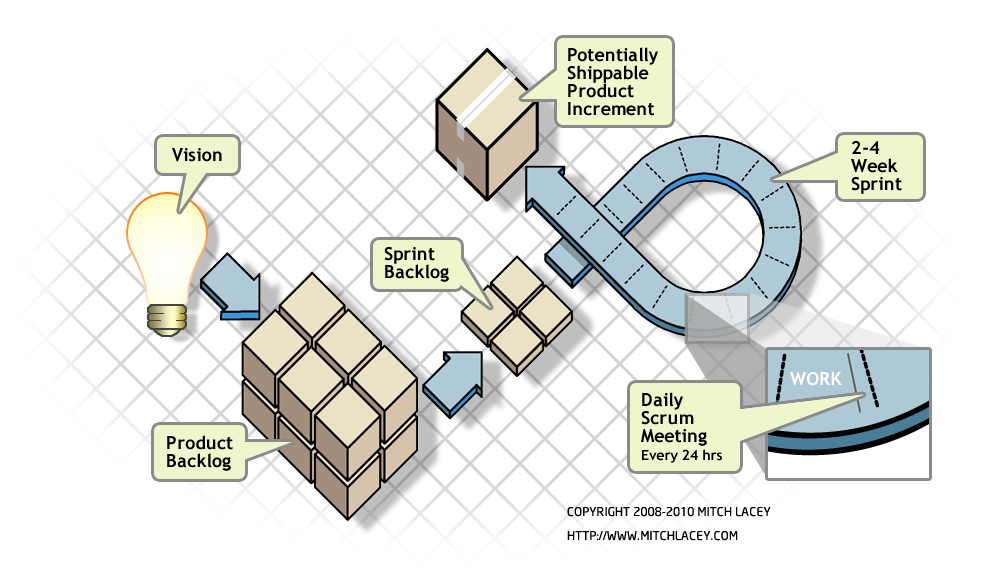
\includegraphics[width=\textwidth]{ScrumFrameworkFlow}
	\caption{Scrum Framework}
	\label{ScrumFramework}
\end{figure*}

Unsere \textbf{Vision} war die in Kapitel \ref{subsubsec:ziel} beschriebene Zielsetzung. Der Dokumentationsaufwand in der Behinderten- und Altenhilfe
soll durch die \EBP verringert werden. Das \textbf{Product Backlog} bildeten die gesamten User Stories, die bei ihrer Erstellung priorisiert wurden.
Das \textbf{Sprint Backlog} bestand in jeder Iteration aus drei bis vier User Stories. Dieses \textbf{Sprint Backlog} wurde in innerhalb einer
\textbf{Sprint} Phase abgearbeitet. Als Zeitraum für einen \textbf{Sprint} waren vier Wochen geplant, so dass nach fünf \textbf{Sprint} Phasen das
Projekt fertig entwickelt sein sollte und vier Wochen als Puffer verbleiben sollten. Zur Visualisierung des \textbf{Product} und \textbf{Sprint
Backlogs} wurden die Werkzeuge der Plattform \url{github.com} genutzt. Die Plattform bietet neben der Versionskontrolle durch das verteilte
Versionsverwaltungswerkzeugs \textit{git} auch die Möglichkeit Meilensteine mit zugehörigen Aufgaben zu definieren und diese einzelnen
Projektteilnehmern zuzuordnen. Das \textbf{Daily Scrum Meeting} wurde nicht in der vom \textit{Scrum Frameworks} vorgesehen Regelmäßigkeit und
Verbindlichkeit durchgeführt. In der ex post Betrachtung stellt sich dies als Fehler heraus. Schwierigkeiten bei der Implementierungen hätten sich
bei regelmäßiger Rücksprache untereinander sicher schneller lösen lassen. Auch eine stärkere Verbindlichkeit gegenüber den Projektzielen hätte sich
durch kontinuierliche Reflexion erzeugen lassen und zu einem besseren Produkt geführt. Eine \textbf{Shippable Product Increment} war nicht das Ziel
einer \textbf{Sprint} Phase. Allerdings sollten die User Stories des jeweiligen \textbf{Sprint Backlogs} am Ende einer \textbf{Sprint} Phase
vollständig umgesetzt sein, inklusive durchlaufener Qualitätssicherung.  
